\documentclass{beamer}
\usepackage[utf8]{inputenc}
\usepackage{graphicx, epsfig}
\usepackage{amsmath,mathrsfs,amsfonts,amssymb}
\usepackage{floatflt}
\usepackage{epic,ecltree}
\usepackage{mathtext}
\usepackage{fancybox}
\usepackage{fancyhdr}
\usepackage{multirow}
\usepackage{enumerate}
\usepackage{epstopdf}
\usepackage{multicol}
\usepackage{algorithm}
\usepackage[noend]{algorithmic}
\usepackage{tikz}
\usepackage{blindtext}
\usepackage{multido}
\usetheme{default}%{Singapore}%{Warsaw}%{Warsaw}%{Darmstadt}
\usecolortheme{default}

\setbeamerfont{title}{size=\Huge}
\setbeamertemplate{footline}[frame number]{}

\setbeamertemplate{section in toc}[sections numbered]

\makeatletter
\newcommand\HUGE{\@setfontsize\Huge{35}{40}}
\makeatother    

\setbeamerfont{title}{size=\HUGE}
\beamertemplatenavigationsymbolsempty

\usetikzlibrary{arrows,shapes,positioning,shadows,trees}

\newcommand\myfootnote[1]{%
  \vspace{-0.5cm}%
  \tikz[remember picture,overlay]
  \draw (current page.south west) +(1in + \oddsidemargin,0.5em)
  node[anchor=south west,inner sep=0pt]{\parbox{\textwidth}{%
      \rlap{\rule{10em}{0.4pt}}\raggedright\scriptsize \textit{#1}}};}

\newcommand\myfootnotewithlink[2]{%
  \vspace{-0.5cm}%
  \tikz[remember picture,overlay]
  \draw (current page.south west) +(1in + \oddsidemargin,0.5em)
  node[anchor=south west,inner sep=0pt]{\parbox{\textwidth}{%
      \rlap{\rule{10em}{0.4pt}}\raggedright\scriptsize\href{#1}{\textit{#2}}}};}

\AtBeginSection[]
      {
      	\begin{frame}{Outline}
      		\tableofcontents[currentsection]
      	\end{frame}
      }
      \AtBeginSubsection[]{
      	\begin{frame}{Outline}
      		\tableofcontents[currentsection,currentsubsection]
      	\end{frame}
}

\newcounter{noscounter} % Используется для nextonslide команды (обнуляется только на новом слайде)
\newcounter{pcounter} % Используется для pause команды (обнуляется после использования eqpause)
\newcounter{diffcounter} % Считает количество pause после формулы

\newcommand{\nextonslide}[1]{%
  \stepcounter{noscounter}% Прибавляем счетчик nextonslide
  \stepcounter{pcounter}% Прибавляем счетчик pause
  \stepcounter{diffcounter}% Прибавляем счетчик diffcounter
  \onslide<\value{noscounter}->{#1}% Отображаем аргумент в скобках на слайде с номером noscounter
}
\newcommand{\resetonslide}{%
    \setcounter{noscounter}{1}% Сбрасываем счетчик nextonslide
    \setcounter{pcounter}{1}% Сбрасываем счетчик pause
    \setcounter{diffcounter}{0}% Сбрасываем счетчик diffcounter
}

\newcommand{\eqpause}{%
  \multido{\i=1+1}{\value{pcounter}}{\pause}% Повторяем pcounter раз команду pause
  \stepcounter{noscounter}% Прибавляем счетчик nextonslide
  \setcounter{pcounter}{1}% Сбрасываем счетчик pause
}

\newcommand{\eqpausediff}{% Вспомогательная команда, запускается автоматически после формул
  \multido{\i=1+1}{\value{diffcounter}}{\pause}% Повторяем diffcounter раз команду pause
  \addtocounter{pcounter}{-\value{diffcounter}}% Вычитаем из pcounter количество сделанных pause
  \setcounter{diffcounter}{0}% Сбрасываем счетчик diffcounter
}

\newcommand\AtEndBoth[2]{% Применяем команду к multline и multline*
  \AtEndEnvironment{#1}{#2}%
  \AtEndEnvironment{#1*}{#2}%
}

\AtEndBoth{align}{\eqpausediff}
\AtEndBoth{equation}{\eqpausediff}
\AtEndBoth{multline}{\eqpausediff}

\addtobeamertemplate{frametitle}{\resetonslide}{}% На каждом слайде сбрасываем счетчики

% latin bold lower
\newcommand{\ba}{\mathbf{a}} 
\newcommand{\bc}{\mathbf{c}} 
\newcommand{\be}{\mathbf{e}} 
\newcommand{\bff}{\mathbf{f}} % \bf - for bold type
\newcommand{\bg}{\mathbf{g}} 
\newcommand{\bh}{\mathbf{h}} 
\newcommand{\bp}{\mathbf{p}} 
\newcommand{\bq}{\mathbf{q}} 
\newcommand{\bt}{\mathbf{t}} 
\newcommand{\bs}{\mathbf{s}} 
\newcommand{\bu}{\mathbf{u}} 
\newcommand{\bv}{\mathbf{v}} 
\newcommand{\bw}{\mathbf{w}} 
\newcommand{\bx}{\mathbf{x}} 
\newcommand{\by}{\mathbf{y}} 
\newcommand{\bz}{\mathbf{z}} 

% latin bold upper
\newcommand{\bA}{\mathbf{A}} 
\newcommand{\bB}{\mathbf{B}} 
\newcommand{\bC}{\mathbf{C}} 
\newcommand{\bG}{\mathbf{G}} 
\newcommand{\bI}{\mathbf{I}} 
\newcommand{\bJ}{\mathbf{J}} 
\newcommand{\bL}{\mathbf{L}} 
\newcommand{\bM}{\mathbf{M}} 
\newcommand{\bP}{\mathbf{P}}
\newcommand{\bQ}{\mathbf{Q}} 
\newcommand{\bR}{\mathbf{R}} 
\newcommand{\bT}{\mathbf{T}} 
\newcommand{\bU}{\mathbf{U}} 
\newcommand{\bV}{\mathbf{V}} 
\newcommand{\bW}{\mathbf{W}} 
\newcommand{\bX}{\mathbf{X}} 
\newcommand{\bY}{\mathbf{Y}} 
\newcommand{\bZ}{\mathbf{Z}} 

% latin cal upper
\newcommand{\cF}{\mathcal{F}} 
\newcommand{\cG}{\mathcal{G}} 
\newcommand{\cI}{\mathcal{I}} 
\newcommand{\cL}{\mathcal{L}} 
\newcommand{\cM}{\mathcal{M}} 
\newcommand{\cN}{\mathcal{N}} 
\newcommand{\cP}{\mathcal{P}} 
\newcommand{\cS}{\mathcal{S}} 
\newcommand{\cT}{\mathcal{T}} 
\newcommand{\cW}{\mathcal{W}} 
\newcommand{\cX}{\mathcal{X}} 
\newcommand{\cZ}{\mathcal{Z}} 

% latin bb upper
\newcommand{\bbE}{\mathbb{E}} 
\newcommand{\bbI}{\mathbb{I}} 
\newcommand{\bbP}{\mathbb{P}} 
\newcommand{\bbR}{\mathbb{R}} 

% greek bold lower
\newcommand{\bepsilon}{\boldsymbol{\epsilon}} 
\newcommand{\btheta}{\boldsymbol{\theta}} 
\newcommand{\blambda}{\boldsymbol{\lambda}} 
\newcommand{\bpi}{\boldsymbol{\pi}} 
\newcommand{\bmu}{\boldsymbol{\mu}} 
\newcommand{\bsigma}{\boldsymbol{\sigma}} 
\newcommand{\bphi}{\boldsymbol{\phi}} 

% greek bold upper
\newcommand{\bSigma}{\boldsymbol{\Sigma}} 

\DeclareMathOperator*{\argmin}{arg\,min}
\DeclareMathOperator*{\argmax}{arg\,max}
\newcommand{\createdgmtitle}[1]{\title[\hbox to 56mm{Deep Generative Models  \hfill\insertframenumber\,/\,\inserttotalframenumber}]
	{\vspace{1cm} \\ \textbf{Deep Generative Models} \\ {\Huge Lecture #1}}
	\author{Roman Isachenko}
	\institute{
		Moscow Institute of Physics and Technology \\
		Yandex School of Data Analysis
	}
	\date{2025, Autumn}
}
\createdgmtitle{1}

\usepackage{tikz}
\usetikzlibrary{arrows,shapes,positioning,shadows,trees}
%--------------------------------------------------------------------------------
\begin{document}
%--------------------------------------------------------------------------------
\begin{frame}[noframenumbering,plain]
%\thispagestyle{empty}
\titlepage
\end{frame}
%=======
\begin{frame}{Generative Models Zoo}
	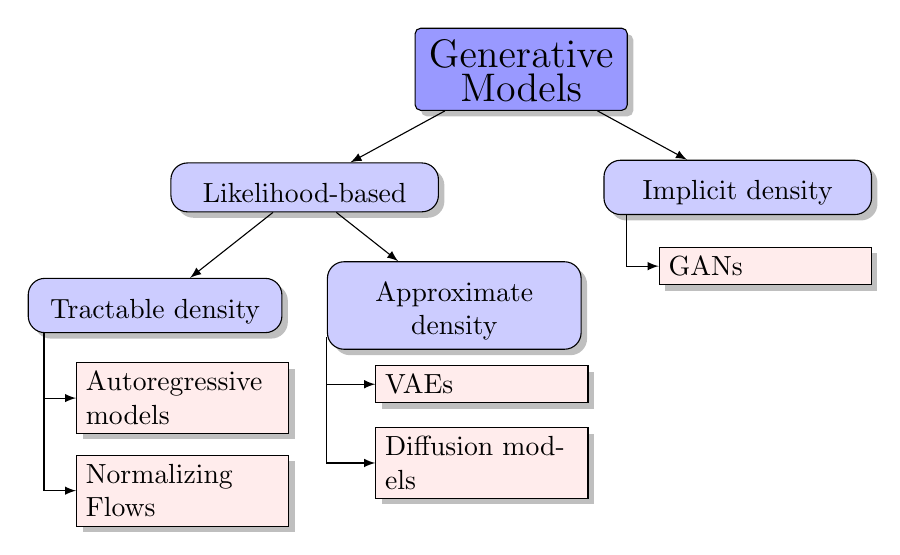
\begin{tikzpicture}[
	 	basic/.style  = {draw, text width=2cm, drop shadow, rectangle},
	 	root/.style   = {basic, rounded corners=2pt, thin, text height=1.1em, text width=7em, align=center, fill=blue!40},
	 	level 1/.style={sibling distance=55mm},
	 	level 2/.style = {basic, rounded corners=6pt, thin, align=center, fill=blue!20, text height=1.1em, text width=9em, sibling distance=38mm},
	 	level 3/.style = {basic, rounded corners=6pt, thin,align=center, fill=blue!20, text width=8.5em},
	 	level 4/.style = {basic, thin, align=left, fill=pink!30, text width=7em},
		edge from parent/.style={->,draw},
		>=latex]
		
		% Root of the tree, level 1
		\node[root] {\Large Generative Models}
		% The first level, as children of the initial tree
		child {node[level 2] (c1) {Likelihood-based}
			child {node[level 3] (c11) {Tractable density}}
			child {node[level 3] (c12) {Approximate density}}
		}
		child {node[level 2] (c2) {Implicit density}};
		
		% Second level, relatively positioned nodes
		\begin{scope}[every node/.style={level 4}]
		\node [below of = c11, yshift=-5pt, xshift=10pt] (c111) {Autoregressive models};
		\node [below of = c111, yshift=-5pt] (c112) {Normalizing Flows};
		
		\node [below of = c12, xshift=10pt] (c121) {VAEs};
		\node [below of = c121] (c122) {Diffusion models};
		
		\node [below of = c2, xshift=10pt] (c21) {GANs};
		\end{scope}
		
		% Lines from each level 1 node to every one of its "children"
		\foreach \value in {1,2}
		\draw[->] (c11.194) |- (c11\value.west);
		
		\foreach \value in {1,2}
		\draw[->] (c12.194) |- (c12\value.west);
		
		\draw[->] (c2.194) |- (c21.west);
		
	\end{tikzpicture}
\end{frame}
%=======
\begin{frame}{Outline}
	\tableofcontents
\end{frame}
%=======
\section{Generative Models Overview}
%=======
\begin{frame}{VAE -- The First Scalable Approach for Image Generation}
    \begin{figure}
        \centering
        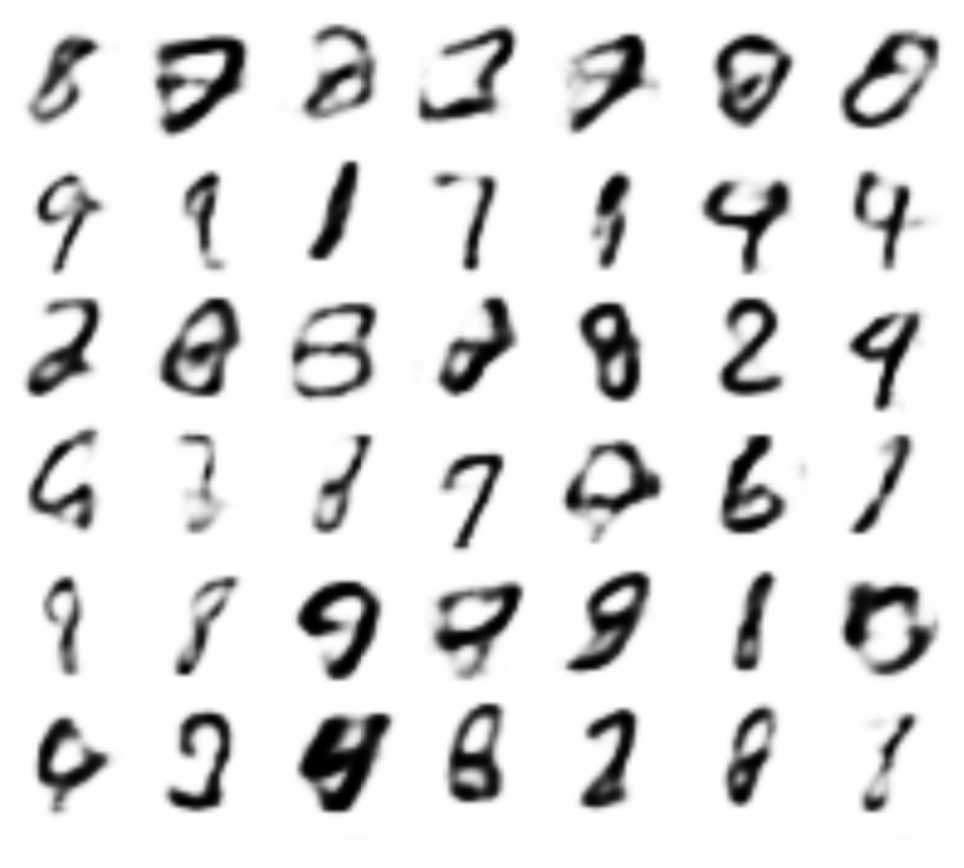
\includegraphics[width=0.8\linewidth]{figs/vae.png}
    \end{figure}
\myfootnotewithlink{https://arxiv.org/abs/1312.6114}{Kingma D. P., Welling M. Auto-Encoding Variational Bayes, 2013}
\end{frame}
%=======
\begin{frame}{DCGAN -- The First Convolutional GAN for Image Generation}
    \begin{figure}
        \centering
        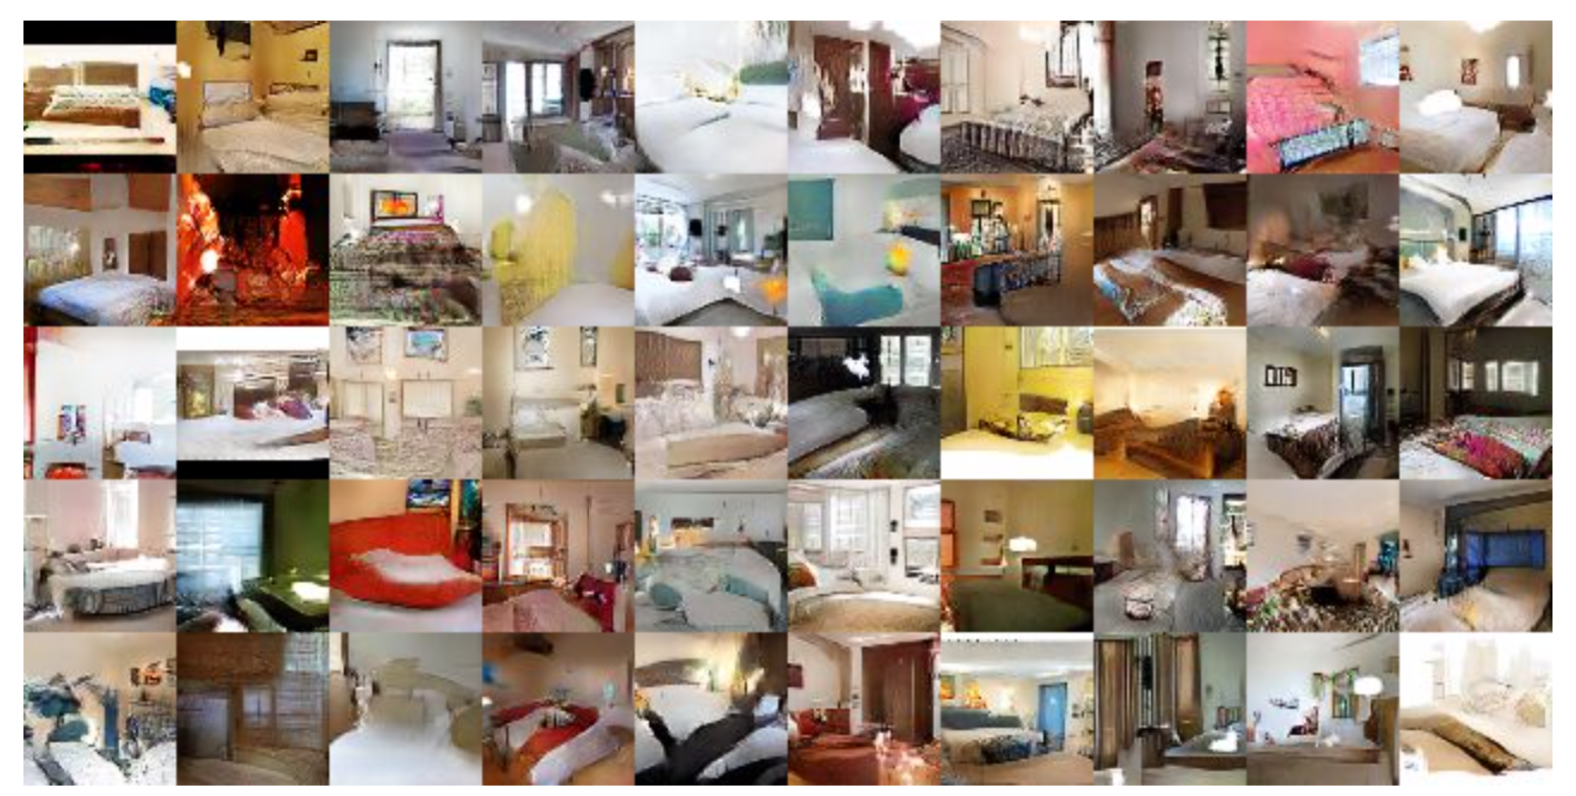
\includegraphics[width=1.0\linewidth]{figs/dcgan.png}
    \end{figure}
\myfootnotewithlink{https://arxiv.org/abs/1511.06434}{Radford A., Metz L., Chintala S. Unsupervised Representation Learning with Deep Convolutional Generative Adversarial Networks, 2015}
\end{frame}
%=======
\begin{frame}{StyleGAN -- High-Quality Face Generation}
	\begin{figure}
		\centering
		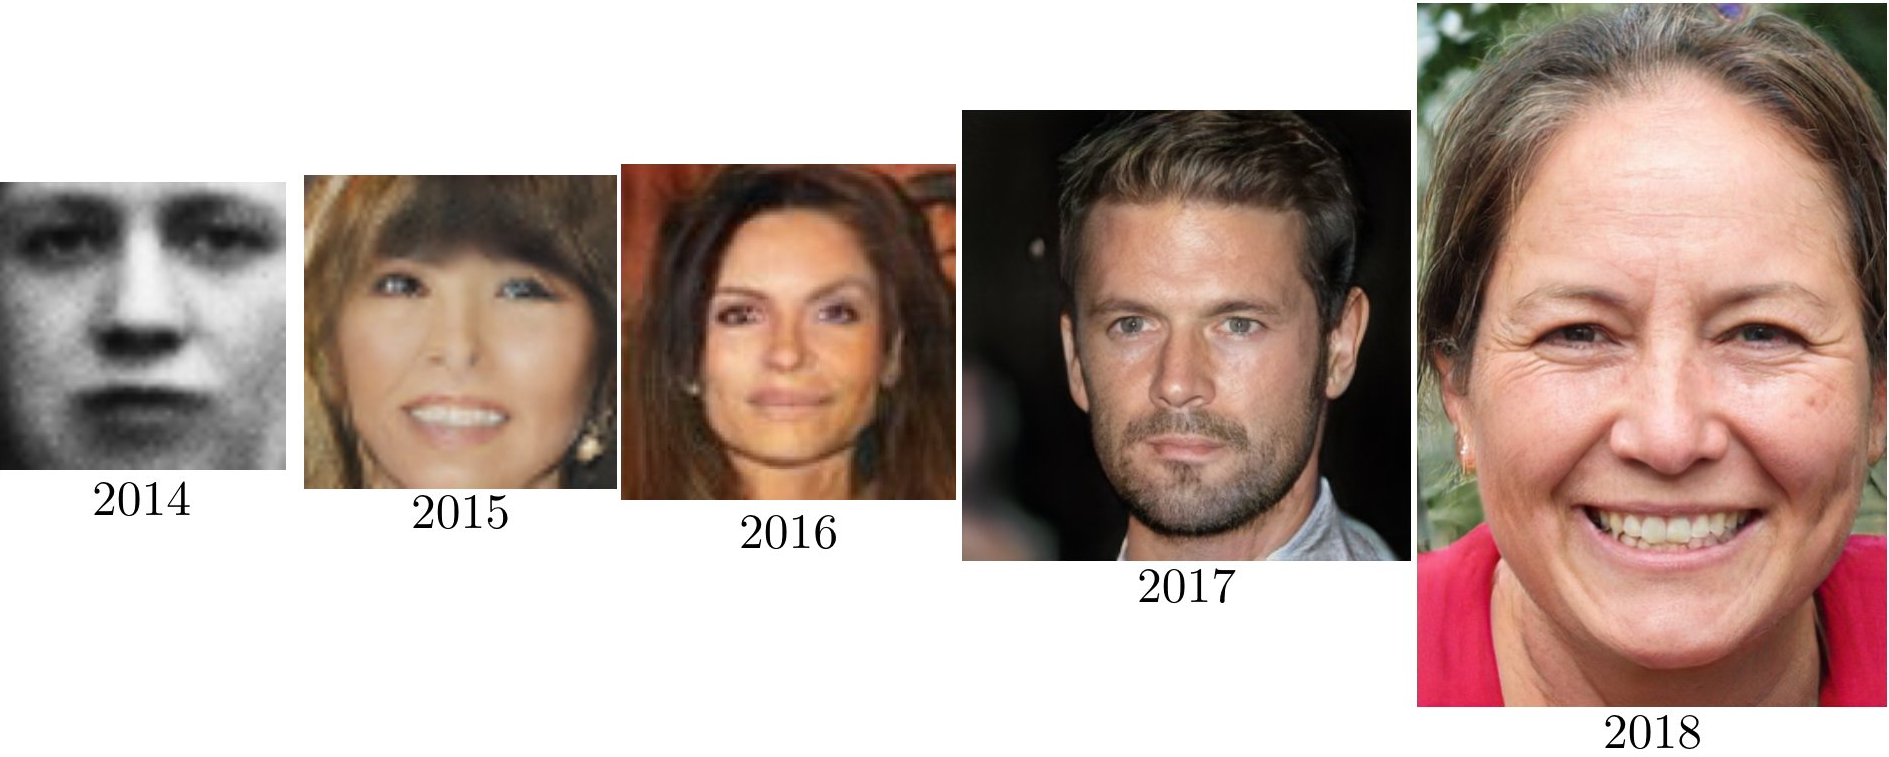
\includegraphics[width=0.85\linewidth]{figs/gan_evolution}
	\end{figure}
	\vspace{-0.2cm}
	\begin{figure}
		\centering
		\includegraphics[width=0.75\linewidth]{figs/stylegan}
	\end{figure}
	\myfootnotewithlink{https://arxiv.org/abs/1812.04948}{Karras T., Laine S., Aila T. A Style-Based Generator Architecture for Generative Adversarial Networks, 2018}
\end{frame}
%=======
\begin{frame}{Language Modeling at Scale}
	\begin{figure}
		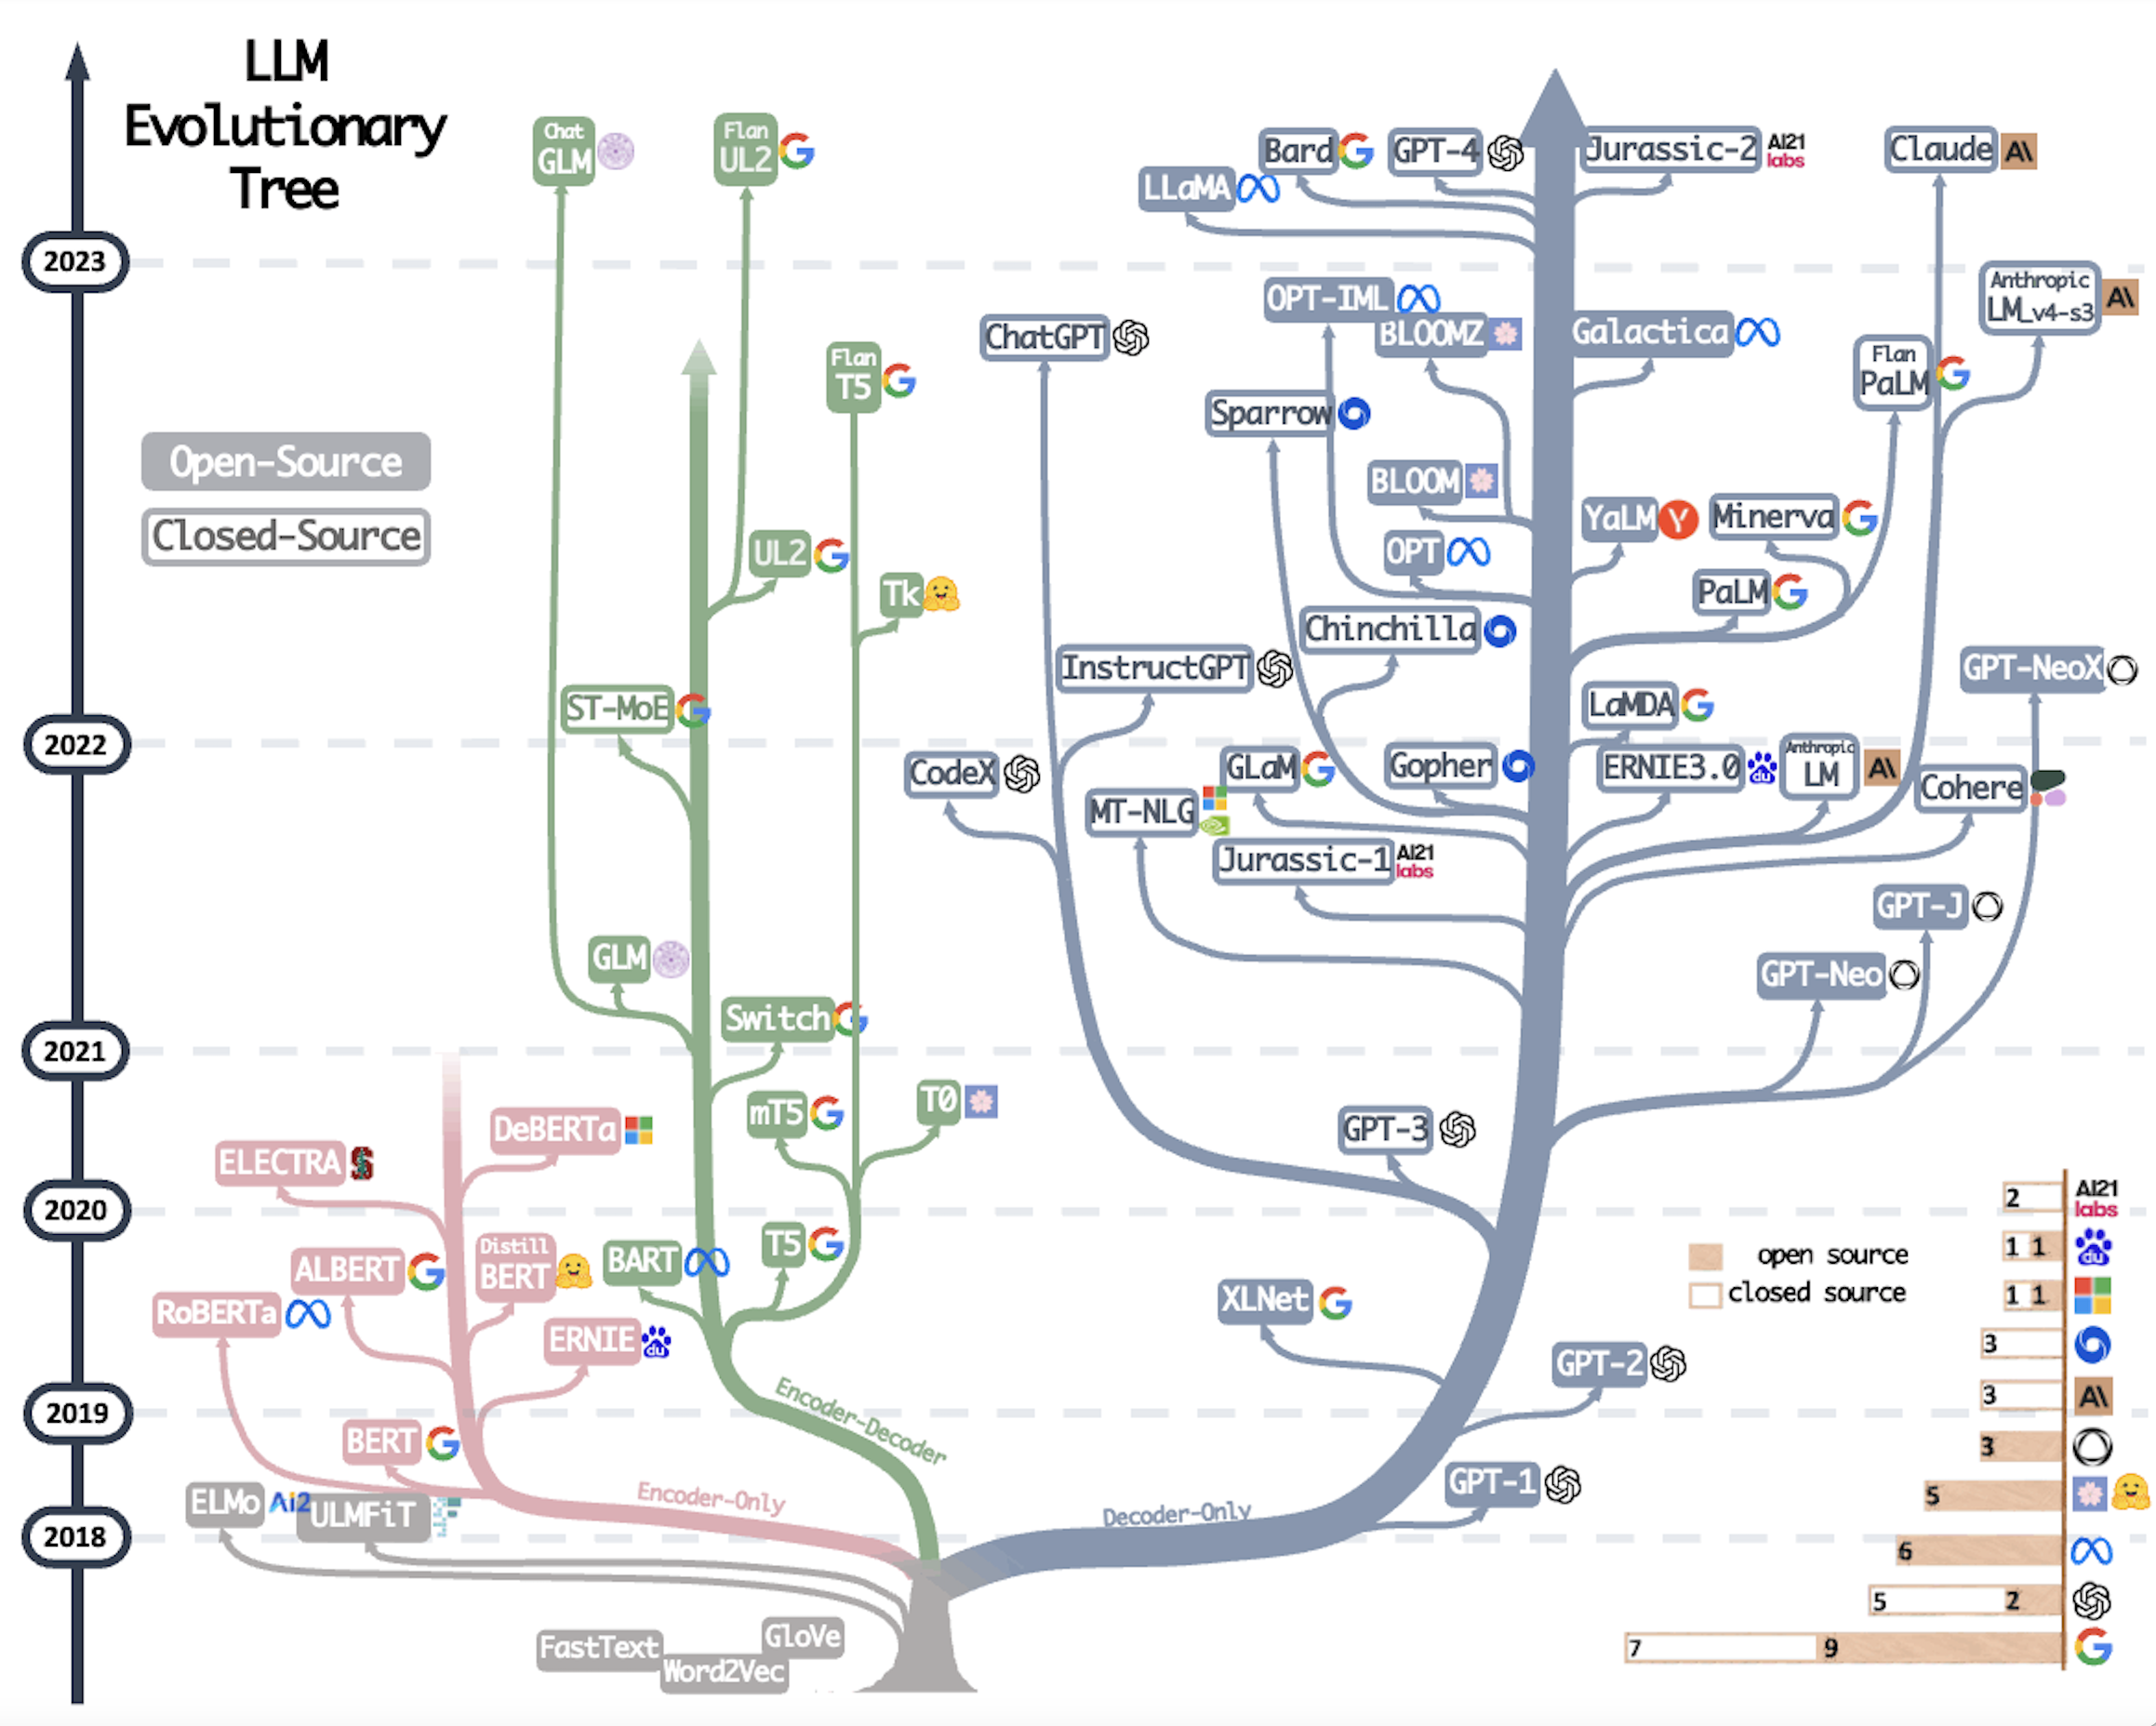
\includegraphics[width=0.85\linewidth]{figs/LLM-Evolutionary-Tree}
	\end{figure}
\myfootnotewithlink{https://blog.biocomm.ai/2023/05/14/open-source-proliferation-llm-evolutionary-tree/}{Image credit: https://blog.biocomm.ai/2023/05/14/open-source-proliferation-llm-evolutionary-tree/}
\end{frame}
%=======
\begin{frame}{Denoising Diffusion Probabilistic Model}
	\begin{figure}
		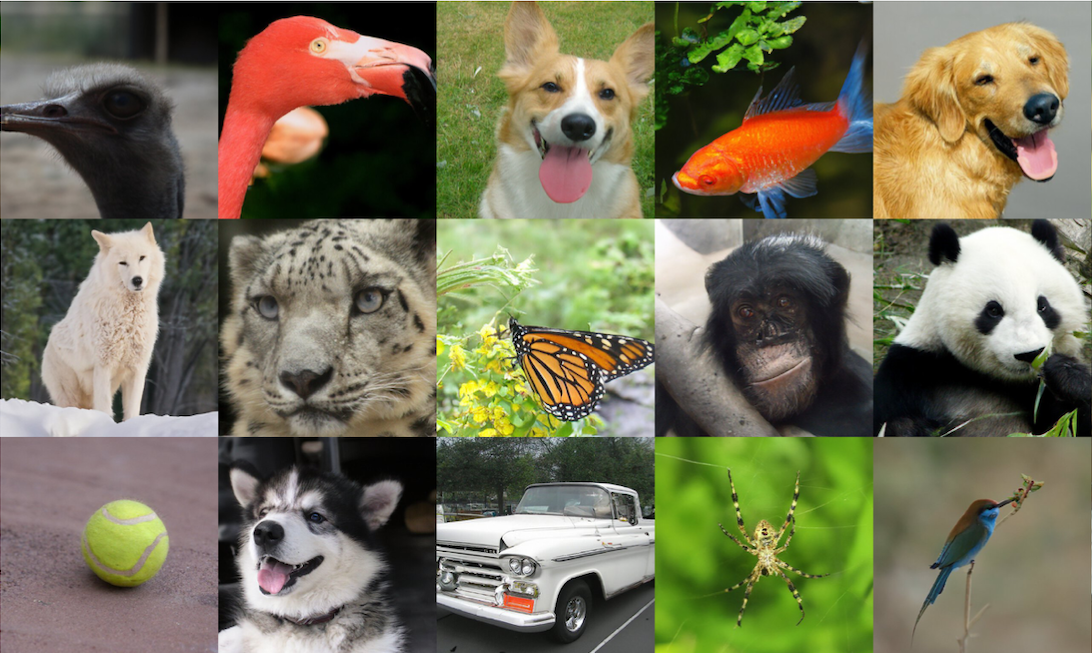
\includegraphics[width=\linewidth]{figs/diffusion_models}
	\end{figure}
	\myfootnotewithlink{https://arxiv.org/abs/2105.05233}{Dhariwal P., Nichol A. Diffusion Models Beat GANs on Image Synthesis, 2021}
\end{frame}
%=======
\begin{frame}{Midjourney -- Impressive Text-to-Image Results}
	\begin{figure}
		\includegraphics[width=\linewidth]{figs/midjourney}
	\end{figure}
	\myfootnotewithlink{https://www.midjourney.com/explore}{Image credit: https://www.midjourney.com/explore}
\end{frame}
%=======
\begin{frame}{Stable Diffusion 3 -- Flow Matching}
		\begin{figure}
			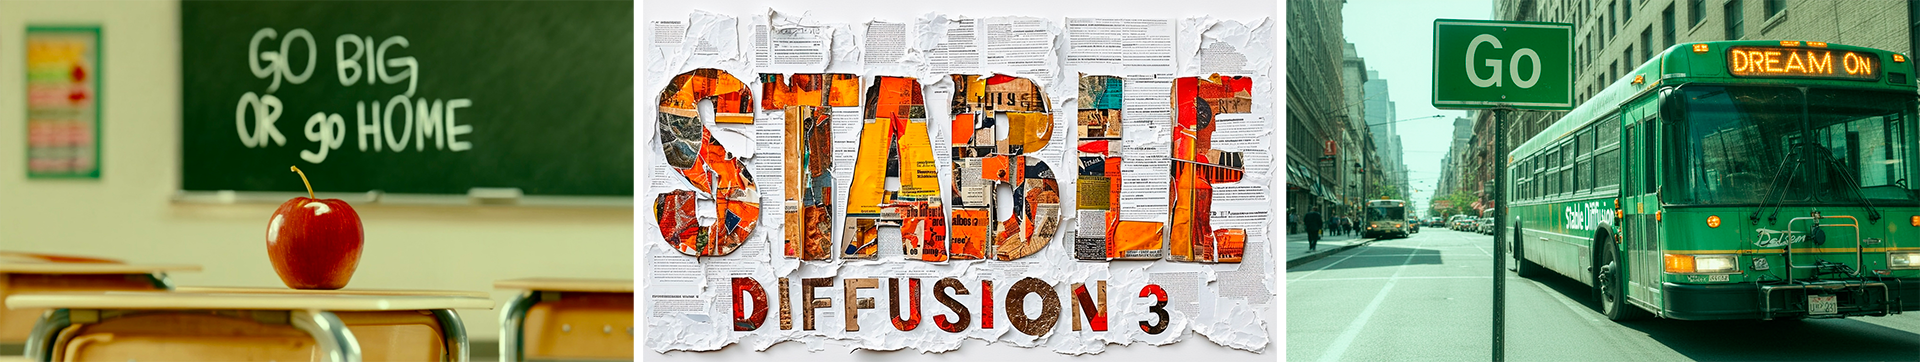
\includegraphics[width=\linewidth]{figs/sd3_1}
		\end{figure}
		\begin{figure}
			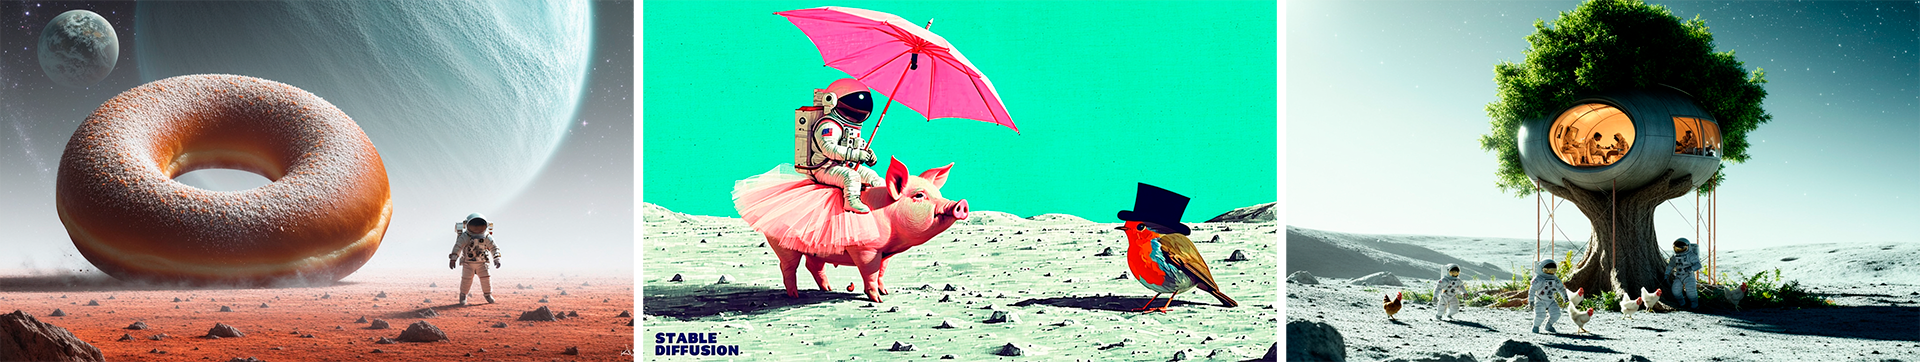
\includegraphics[width=\linewidth]{figs/sd3_2}
		\end{figure}
		\myfootnotewithlink{https://stability.ai/news/stable-diffusion-3}{Image credit: https://stability.ai/news/stable-diffusion-3}
\end{frame}
%=======
\begin{frame}{Sora -- Video Generation}
		\begin{figure}
			\includegraphics[width=\linewidth]{figs/sora}
		\end{figure}
		\myfootnotewithlink{https://openai.com/index/sora}{Image credit: https://openai.com/index/sora}
\end{frame}
%=======
\section{Course Tricks}
%=======
\begin{frame}{Course Tricks 1}
	\begin{block}{Log-Derivative Trick}
		Let $f: \bbR^m \rightarrow \bbR$ be a differentiable function.
		$$
			\nabla \log f(\bx) = \frac{1}{f(\bx)} \cdot \nabla f(\bx).
		$$
		\vspace{-0.5cm}
	\end{block}
	\begin{block}{Jensen's Inequality}
		Let $\bx \in \bbR^m$ be a continuous random variable with density $p(\bx)$, and $f: \bbR^m \rightarrow \bbR$ be a convex function. Then
		$$
			\bbE [f(\bx)] \geq f(\bbE[\bx]).
		$$
		\vspace{-0.7cm}
	\end{block}
	\begin{block}{Monte Carlo Estimation}
		Let $\bx \in \bbR^m$ be a continuous random variable with density $p(\bx)$ and $\bff: \bbR^m \rightarrow \bbR^d$ be a vector-valued function. Then 
		$$
			\bbE_{p(\bx)} \bff(\bx) = \int p(\bx) \bff(\bx) d \bx \approx \frac{1}{n} \sum_{i=1}^n \bff(\bx_i), \quad 
			\text{where } \bx_i \sim p(\bx).
		$$
		\vspace{-0.4cm}
	\end{block}
\end{frame}
%=======
\begin{frame}{Course Tricks 2}
	\begin{block}{Change of Variables Theorem (CoV)}
		Let $\bx$ be a continuous random variable with density $p(\bx)$, and $\bff: \bbR^m \rightarrow \bbR^m$ be a differentiable, \textbf{invertible} function. If $\by = \bff(\bx)$, then
		$$
			p(\by) = p(\bx) \left|\det \left(  \frac{\partial \bx}{\partial \by} \right) \right| = p(\bff^{-1}(\by)) \left|\det \left(  \frac{\partial \bff^{-1}(\by)}{\partial \by} \right) \right|.
		$$
		\vspace{-0.5cm}
	\end{block}
	\begin{block}{Proof (1D)}
		Assume $f$ is a monotonically increasing function.
		$$
			F_Y(y) = P(Y \leq y) = P(x \leq f^{-1}(y)) = F_X(f^{-1}(y))
		$$
		$$
			p(y) = \frac{dF_Y(y)}{dy} = \frac{dF_X(f^{-1}(y))}{dy} = \frac{dF_X(x)}{dx} \frac{df^{-1}(y)}{dy} =  p(x) \frac{df^{-1}(y)}{dy}
		$$
	\end{block}
\end{frame}
%=======
\begin{frame}{Course Tricks 3}
	\begin{block}{Law of the Unconscious Statistician (LOTUS)}
		Let $\bx \in \bbR^m$ be a continuous random variable with density $p(\bx)$ and let $\bff: \bbR^m \rightarrow \bbR^m$ be a measurable function. If $\by = \bff(\bx)$, then
		$$
			\bbE_{p(\by)} \bg(\by) = \int p(\by) \bg(\by) d\by = \int p(\bx) \bg(\bff(\bx)) d\bx = \bbE_{p(\bx)} \bg(\bff(\bx)).
		$$
		\vspace{-0.4cm}
	\end{block}
	\begin{block}{Dirac Delta Function}
		We can treat any deterministic variable $\bx_0$ as a random variable with density $p(\bx) = \delta(\bx - \bx_0)$. 
		\vspace{-0.3cm}
		$$
			\delta(\bx) = 
			\begin{cases}
				+\infty, \quad \bx = 0; \\
				0, \quad \bx \neq 0;
			\end{cases} \, 
			\int \delta(\bx) d\bx = 1.
		$$
		$$
			\bbE_{p(\bx)}\bff(\bx) = \int \delta (\bx - \bx_0) \bff(\bx) d\bx = \bff(\bx_0).
		$$
	\end{block}
\end{frame}
%=======
\section{Problem Statement}
%=======
\begin{frame}{Problem statement}
	We are given i.i.d. samples $\{\bx_i\}_{i=1}^n \in \bbR^m$ from \textbf{unknown} distribution $\pi(\bx)$.
	
	\begin{block}{Objective}
		Our goal is to learn a distribution $\pi(\bx)$ that enables: 
		\begin{itemize}
		    \item evaluating $\pi(\bx)$ for new data (how likely is an object $\bx$?)~-- \textbf{density estimation};
		    \item sampling from $\pi(\bx)$ (to generate new objects $\bx \sim \pi(\bx)$)~-- \textbf{generation}.
		\end{itemize}
	\end{block}
	\begin{block}{Challenge}
		The data is complex and high-dimensional. For example, a dataset of images resides in the space $\bbR^{\text{width} \times \text{height} \times \text{channels}}$. The curse of dimensionality prevents us from finding the exact density $\pi(\bx)$. 
	\end{block}
\end{frame}
%=======
\begin{frame}{Histogram as a Generative Model}
	
	\begin{minipage}[t]{0.6\columnwidth}
	    Assume $x \sim \textrm{Categorical}(\bpi)$. The histogram is completely determined by
		$$
		    \hat{\pi}_k = \hat{\pi}(x = k) = \frac{\sum_{i=1}^n [x_i = k]}{n}.
		$$
		\textbf{The curse of dimensionality:} the number of bins grows exponentially. \\
		\end{minipage}%
		\begin{minipage}[t]{0.4\columnwidth}
	    \begin{figure}[h]
	        \centering
	        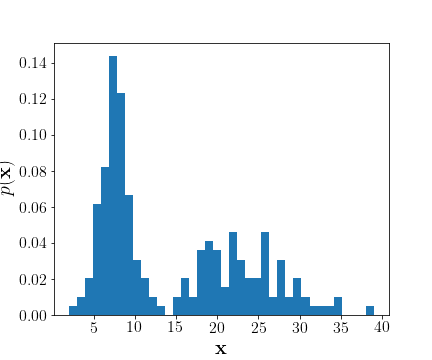
\includegraphics[width=\linewidth]{figs/histogram.png}
	    \end{figure}
	\end{minipage}
	\textbf{MNIST example}: 28x28 grayscale images, where each image is $\bx = (x_1, \dots, x_{784})$, and $x_i \in \{0, 1\}$. 
	$$
	    \pi(\bx) = \pi(x_1) \cdot \pi(x_2 | x_1) \cdot \dots \cdot \pi(x_m | x_{m-1}, \dots, x_1).
	$$
	Hence, a full histogram would require $2^{28 \times 28} - 1$ parameters to specify~$\pi(\bx)$. \\
	\textbf{Question:} How many parameters do we need in these cases?
	\begin{align*}
	    \pi(\bx) &= \pi(x_1) \cdot \pi(x_2)\cdot \dots \cdot \pi(x_m); \\
	    \pi(\bx) &= \pi(x_1) \cdot \pi(x_2 | x_1) \cdot \dots \cdot \pi(x_m | x_{m-1}).
	\end{align*}
\end{frame}
%=======
\begin{frame}{Problem Statement: Conditional Models}
	\begin{block}{Conditional Model}
		In practice, a common task is to construct a conditional model~$\pi(\bx | \by)$. 
		\begin{itemize}
			\item $\by = \emptyset$, $\bx$ -- image $\Rightarrow$ unconditional image model.
			\item $\by$ -- class label, $\bx$ -- image $\Rightarrow$ class-conditional image model.
			\item $\by$ -- text prompt, $\bx$ -- image $\Rightarrow$ text-to-image model.
			\item $\by$ -- image, $\bx$ -- image $\Rightarrow$ image-to-image model.
			\item $\by$ -- image, $\bx$ -- text $\Rightarrow$ image-to-text model (image captioning).
			\item $\by$ -- English text, $\bx$ -- Russian text $\Rightarrow$ sequence-to-sequence model (machine translation).
			\item $\by$ -- sound, $\bx$ -- text $\Rightarrow$ speech-to-text model (automatic speech recognition).
			\item $\by$ -- text, $\bx$ -- sound $\Rightarrow$ text-to-speech model.
		\end{itemize}
	\end{block}
\end{frame}
%=======
\section{Divergence Minimization Framework}
%=======
\begin{frame}{Divergences}
	\begin{itemize}
	\item Fix a probabilistic model $p(\bx | \btheta)$~-- a family of parameterized distributions. \\
	\item Instead of searching for the true $\pi(\bx)$ among all possible probability distributions, we instead learn a function approximation $p(\bx | \btheta) \approx \pi(\bx)$.
	\end{itemize}
	\begin{block}{What is a Divergence?}
		Let $\cP$ be the set of all probability distributions. A function $D: \cP \times \cP \rightarrow \bbR$ is called a divergence if 
		\begin{itemize}
			\item $D(\pi || p) \geq 0$ for all $\pi, p \in \cP$;
			\item $D(\pi || p) = 0$ if and only if $\pi \equiv p$.
		\end{itemize}
	\end{block}
	\begin{block}{Divergence Minimization Problem}
		\vspace{-0.3cm}
		$$
		\min_{\btheta} D(\pi || p)
		$$
		where $\pi(\bx)$ is the true data distribution and $p(\bx | \btheta)$ is our model distribution.
	\end{block}
\end{frame}
%=======
\begin{frame}{Forward KL vs. Reverse KL (Kullback-Leibler Divergence)}
	\begin{block}{Forward KL}
		\vspace{-0.2cm}
		$$
		KL(\pi || p) = \int \pi (\bx) \log \frac{\pi(\bx)}{p(\bx | \btheta)} d \bx \rightarrow \min_{\btheta}
		$$
	\end{block}
	\begin{block}{Reverse KL}
		\vspace{-0.2cm}
		$$
		KL(p || \pi) = \int p (\bx| \btheta) \log \frac{p(\bx| \btheta)}{\pi(\bx)} d \bx \rightarrow \min_{\btheta}
		$$
	\end{block}
	What is the practical difference between these two formulations?
	
	\begin{block}{Maximum Likelihood Estimation (MLE)}
	Let $\{\bx_i\}_{i=1}^n$ denote the set of observed i.i.d. samples.
		\vspace{-0.3cm}
		$$
		\btheta^* = \argmax_{\btheta} \prod_{i=1}^n p(\bx_i | \btheta) = \argmax_{\btheta} \sum_{i=1}^n \log p(\bx_i | \btheta).
		$$
	\end{block}
\end{frame}
%=======
\begin{frame}{Forward KL vs. Reverse KL: MLE as Forward KL}
	\begin{block}{Forward KL}
		\vspace{-0.5cm}
		\begin{align*}
			KL(\pi || p) &= \int \pi(\bx) \log \frac{\pi(\bx)}{p(\bx | \btheta)} d\bx \\
			&= {\color{violet}\int \pi (\bx) \log \pi(\bx) d \bx} - {\color{teal}\int \pi (\bx) \log p(\bx | \btheta) d \bx} \\
			&= - {\color{teal}\bbE_{\pi(\bx)} \log p(\bx | \btheta)} + {\color{violet}\text{const}} \\
			& \approx - \frac{1}{n} \sum_{i=1}^n \log p(\bx_i | \btheta) + \text{const} \rightarrow \min_{\btheta}.
		\end{align*}
		\vspace{-0.5cm}
	\end{block}
	Maximum likelihood estimation is equivalent to minimizing the Monte Carlo estimate of the forward KL divergence.
	\begin{block}{Reverse KL}
		\vspace{-0.5cm}
		\begin{align*}
			KL(p || \pi) &= \int p(\bx | \btheta) \log \frac{p(\bx | \btheta)}{\pi(\bx)} d \bx \\
			&= \bbE_{p(\bx | \btheta)} \left[\log p(\bx | \btheta) - \log \pi(\bx)\right] \rightarrow \min_{\btheta}
		\end{align*}
		\vspace{-0.7cm}
	\end{block}
\end{frame}
%=======
\section{Autoregressive Modeling}
%=======
\begin{frame}{Generative Models Zoo}
	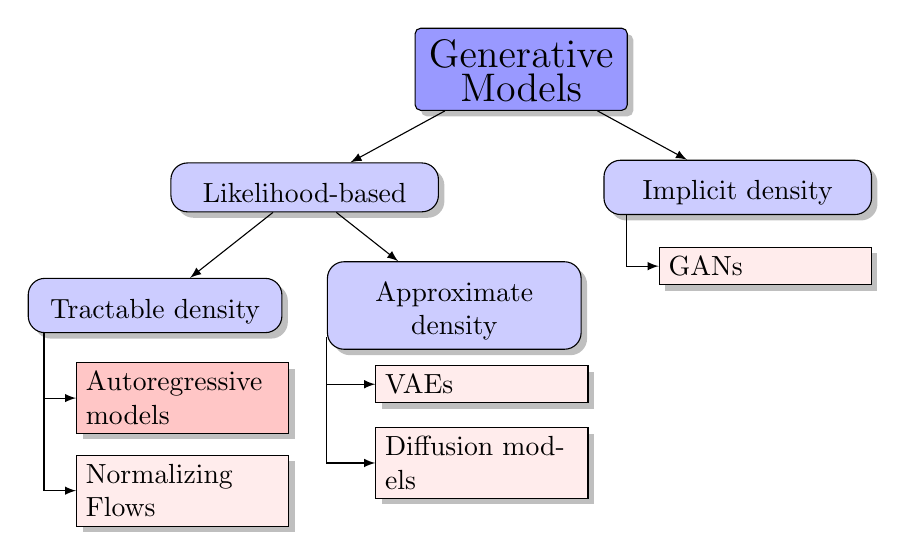
\begin{tikzpicture}[
		basic/.style  = {draw, text width=2cm, drop shadow, rectangle},
		root/.style   = {basic, rounded corners=2pt, thin, text height=1.1em, text width=7em, align=center, fill=blue!40},
		level 1/.style={sibling distance=55mm},
		level 2/.style = {basic, rounded corners=6pt, thin, align=center, fill=blue!20, text height=1.1em, text width=9em, sibling distance=38mm},
		level 3/.style = {basic, rounded corners=6pt, thin,align=center, fill=blue!20, text width=8.5em},
		level 4/.style = {basic, thin, align=left, fill=pink!30, text width=7em},
		level 5/.style = {basic, thin, align=left, fill=pink!90, text width=7em},
		edge from parent/.style={->,draw},
		>=latex]
		
		% Root of initial tree, level 1
		\node[root] {\Large Generative Models}
		% The first level, as children of the initial tree
		child {node[level 2] (c1) {Likelihood-based}
			child {node[level 3] (c11) {Tractable density}}
			child {node[level 3] (c12) {Approximate density}}
		}
		child {node[level 2] (c2) {Implicit density}};
		
		% Second level, relatively positioned nodes
		\begin{scope}[every node/.style={level 5}]
			\node [below of = c11, yshift=-5pt, xshift=10pt] (c111) {Autoregressive models};
		\end{scope}
		
		% Second level, relatively positioned nodes
		\begin{scope}[every node/.style={level 4}]
			\node [below of = c111, yshift=-5pt] (c112) {Normalizing Flows};
			
			\node [below of = c12, xshift=10pt] (c121) {VAEs};
			\node [below of = c121] (c122) {Diffusion models};
			
			\node [below of = c2, xshift=10pt] (c21) {GANs};
		\end{scope}
		
		% Lines from each level 1 node to every one of its "children"
		\foreach \value in {1,2}
		\draw[->] (c11.194) |- (c11\value.west);
		
		\foreach \value in {1,2}
		\draw[->] (c12.194) |- (c12\value.west);
		
		\draw[->] (c2.194) |- (c21.west);
		
	\end{tikzpicture}
\end{frame}
%=======
\begin{frame}{Autoregressive Modeling}
    \begin{block}{MLE Problem}
	    \vspace{-0.4cm}
	    $$
	        \btheta^* = \argmax_{\btheta} \prod_{i=1}^n p(\bx_i | \btheta) = \argmax_{\btheta} \sum_{i=1}^n \log p(\bx_i | \btheta).
	    $$
	    \vspace{-0.5cm}
    \end{block}
    \begin{itemize}
        \item We seek to solve this maximization using gradient-based optimization.
        \item Thus, we need efficient computation of $\log p(\bx | \btheta)$ and its gradient $\frac{\partial \log p(\bx | \btheta)}{\partial \btheta}$.
    \end{itemize}
    \begin{block}{Likelihood as a Product of Conditionals}
    Let $\bx = (x_1, \dots, x_m)$, $\bx_{1:j} = (x_1, \dots, x_j)$. Then 
    $$
        p(\bx | \btheta) = \prod_{j=1}^m p(x_j | \bx_{1:j - 1}, \btheta); \quad 
        \log p(\bx | \btheta) = {\color{violet}\sum_{j=1}^m \log p(x_j | \bx_{1:j - 1}, \btheta)}.
    $$
    \end{block}
    \vspace{-0.5cm}
	 $$
	     \btheta^* =  \argmax_{\btheta} \sum_{i=1}^n \left[{\color{violet} \sum_{j=1}^m \log p(x_{ij} | \bx_{i, 1:j - 1}, \btheta)}\right]
	 $$
\end{frame}
%=======
\begin{frame}{Autoregressive Models}
    $$
    \log p(\bx| \btheta) = \sum_{j=1}^m \log p(x_j | \bx_{1:j - 1}, \btheta)
    $$
    \begin{itemize}
	    \item Sampling is sequential:
	    \begin{itemize}
    		\item sample $\hat{x}_1 \sim p(x_1 | \btheta)$;
    		\item sample $\hat{x}_2 \sim p(x_2 | \hat{x}_1, \btheta)$;
    		\item $\dots$
    		\item sample $\hat{x}_m \sim p(x_m | \hat{\bx}_{1:m-1}, \btheta)$;
    		\item The generated object is $\hat{\bx} = (\hat{x}_1, \hat{x}_2, \dots, \hat{x}_m)$.
    	\end{itemize}
        \item Each conditional $p(x_j | \bx_{1:j - 1}, \btheta)$ can be modeled by a neural network.
        \item Modeling all conditionals separately is infeasible. Sharing parameters $\btheta$ across all conditionals alleviates this issue.
    \end{itemize}
\end{frame}
%=======
\begin{frame}{Autoregressive Models: MLP}
	For large $j$, the conditional distribution $p(x_j | \bx_{1:j - 1}, \btheta)$ can become intractable. Furthermore, the history $\bx_{1:j-1}$ has variable length.
	\begin{block}{Markov Assumption}
		\vspace{-0.5cm}
		$$
			p(x_j | \bx_{1:j - 1}, \btheta) = p(x_j | \bx_{j - d:j - 1}, \btheta), \quad d \text{ is a fixed model parameter}.
		$$
	\end{block}
	\vspace{-0.5cm}
	\begin{block}{Example}
		\begin{minipage}[t]{0.39\columnwidth}
			{\small
			\begin{itemize}
				\item $d = 2$;
				\item $x_j \in \{0, 255\}$;
				\item $\bh_j = \mathrm{MLP}_{\btheta}(x_{j - 1}, x_{j - 2})$;
				\item $\bpi_j = \mathrm{softmax}(\bh_j)$;
				\item $p(x_j | x_{j - 1}, x_{j - 2}, \btheta) = \mathrm{Categorical}(\bpi_j)$.
			\end{itemize}
			}
		\end{minipage}%
		\begin{minipage}[t]{0.61\columnwidth}
			 \begin{figure}
			   \centering
			   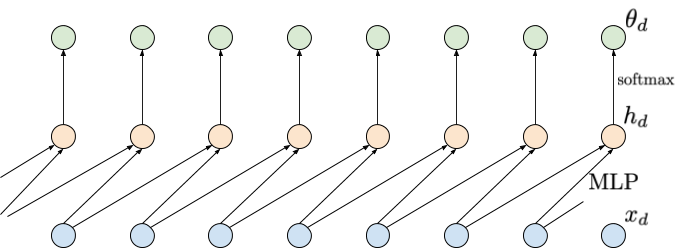
\includegraphics[width=1.0\linewidth]{figs/sequential_MLP}
			 \end{figure}
			 Is it possible to model continuous distributions instead of discrete ones?
		\end{minipage}
	\end{block}
	 \myfootnotewithlink{https://jmtomczak.github.io/blog/2/2\_ARM.html}{Image credit: https://jmtomczak.github.io/blog/2/2\_ARM.html}
\end{frame}
%=======
\begin{frame}{Autoregressive Models: LLM}
	$$
		p(x_j | \bx_{1:j - 1}, \btheta) = p(x_j | \bx_{j - d:j - 1}, \btheta), \quad d \text{ is the context window}.
	$$
	 \begin{figure}
		   \centering
		   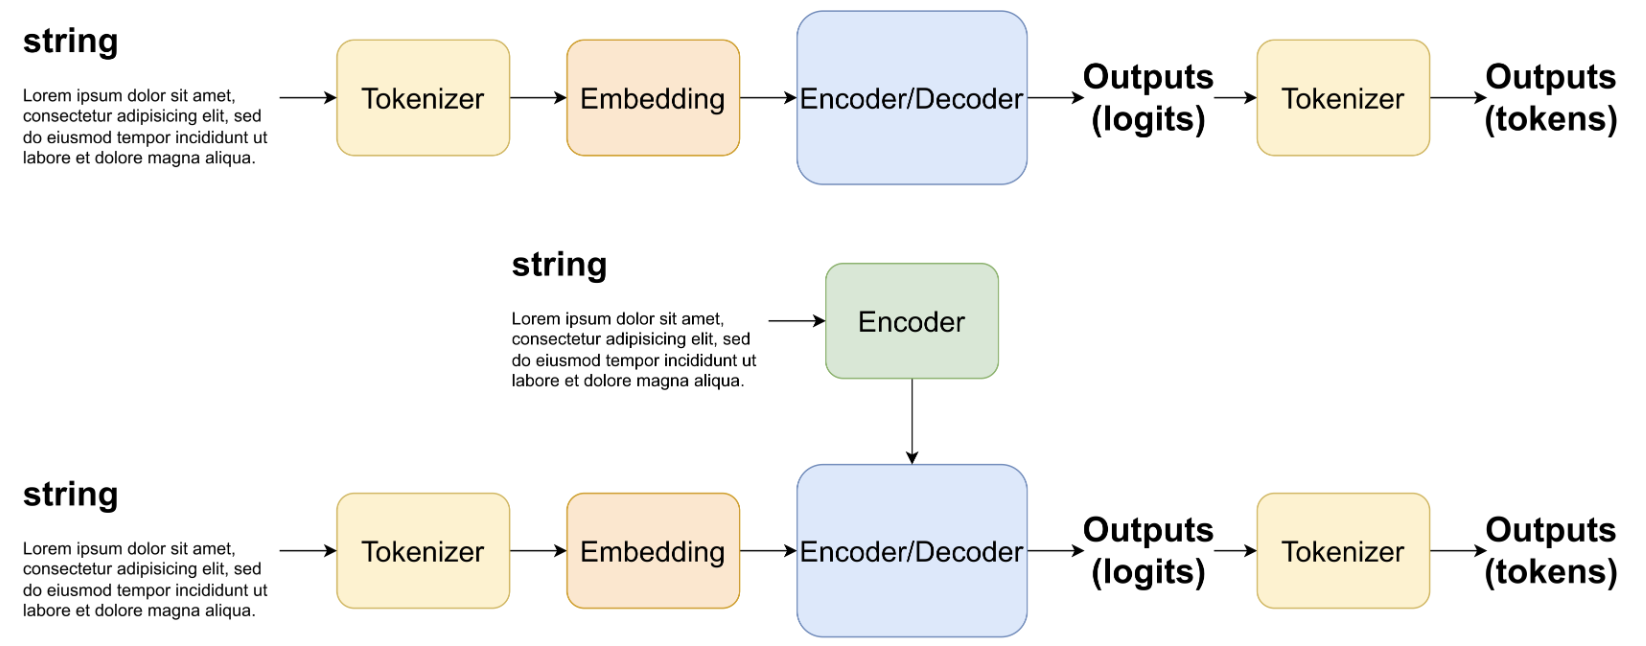
\includegraphics[width=1.0\linewidth]{figs/llm_modeling}
	 \end{figure}
	 \myfootnotewithlink{https://jmtomczak.github.io/blog/20/20\_llms.html}{Image credit: https://jmtomczak.github.io/blog/20/20\_llms.html}
\end{frame}
%=======
\begin{frame}{Autoregressive Models for Images}
	How can we model the distribution $\pi(\bx)$ over natural images?
	$$
  		p(\bx | \btheta) = \prod_{j=1}^{\text{width} \times \text{height}} p(x_j|\bx_{1:j-1}, \btheta).
	$$
	\begin{minipage}[t]{0.5\columnwidth}
		\vspace{0.5cm}
		\begin{itemize}
			\item We must specify an ordering of image pixels. Raster scan order is the most straightforward choice.
		    \item RGB channel dependencies can also be explicitly modeled.
		\end{itemize}
	\end{minipage}%
	\begin{minipage}[t]{0.5\columnwidth}
		\begin{figure}
			\centering
   			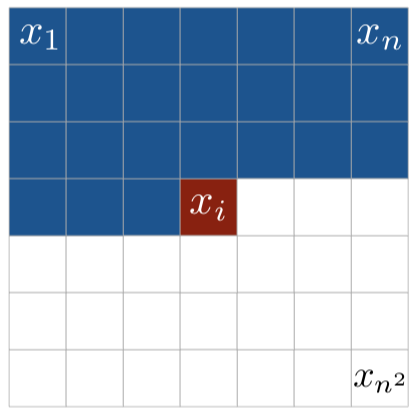
\includegraphics[width=0.9\linewidth]{figs/pixelcnn1.png}
		\end{figure}
	\end{minipage}
	\myfootnotewithlink{https://arxiv.org/abs/1601.06759}{Oord A., Kalchbrenner N., Kavukcuoglu K. Pixel Recurrent Neural Networks, 2016}
\end{frame}
%=======
\begin{frame}{Autoregressive Models: ImageGPT}
	\begin{figure}
		\centering
  			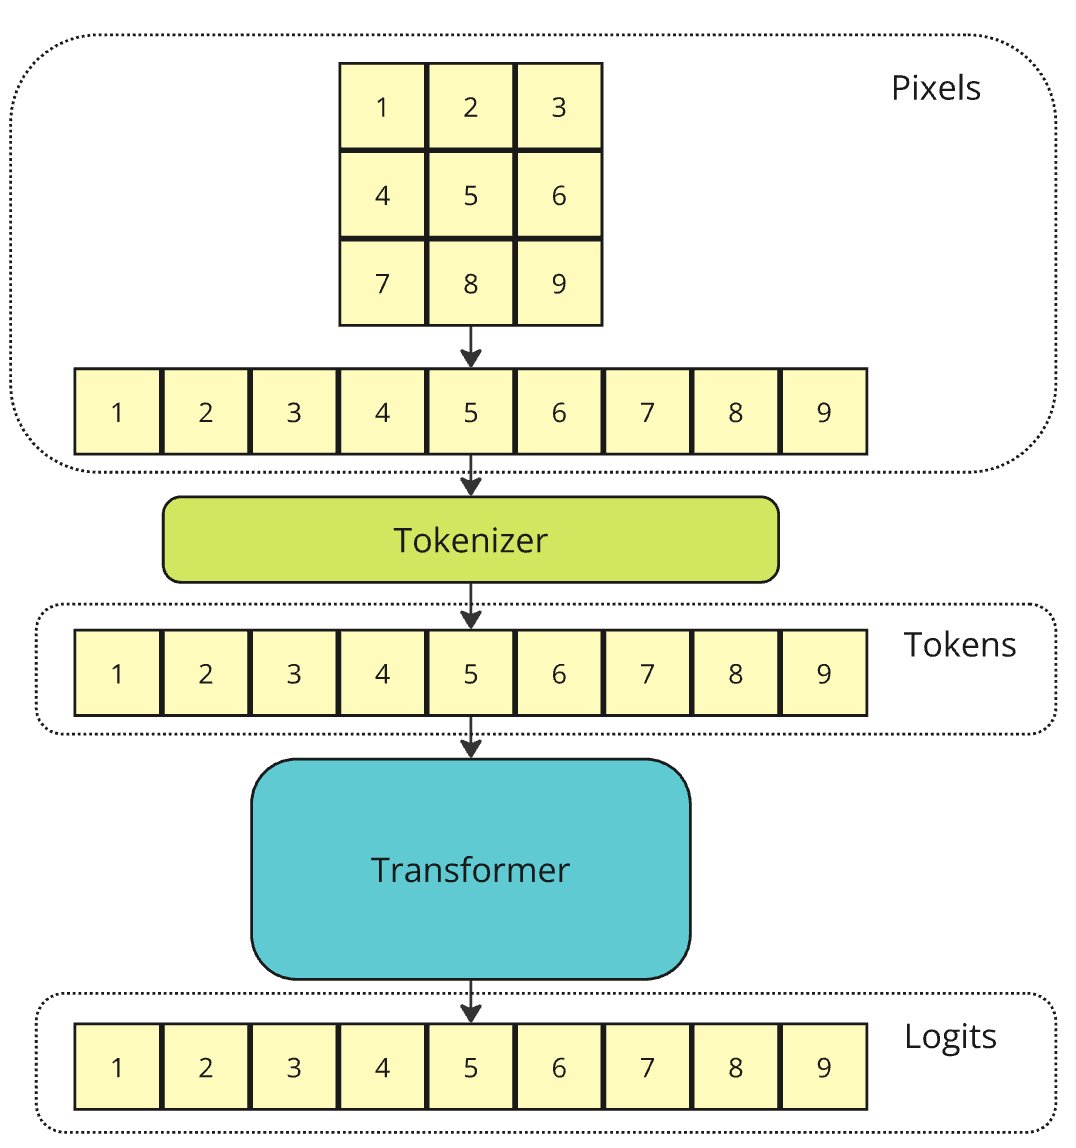
\includegraphics[width=0.65\linewidth]{figs/imagegpt.png}
	\end{figure}
	\myfootnotewithlink{https://cdn.openai.com/papers/Generative_Pretraining_from_Pixels_V2.pdf}{Chen M. et al. Generative Pretraining from Pixels, 2020}
\end{frame}
%=======
\begin{frame}{Summary}
    \begin{itemize}
    	\item We aim to approximate the data distribution for both density estimation and generation of new samples.
    	\vfill
    	\item Divergence minimization provides a general framework to fit a model distribution to the real data distribution.
    	\vfill
    	\item Minimizing the forward KL is equivalent to solving the MLE problem.
    	\vfill
    	\item Autoregressive models decompose the joint distribution into a sequence of conditionals.
    	 \vfill
        \item Sampling from autoregressive models is straightforward, but inherently sequential.
        \vfill
        \item To evaluate the density, multiply all conditionals $p(x_j | \bx_{1:j - 1}, \btheta)$.
        \vfill
     	\item ImageGPT applies the transformer to raster-ordered image pixels.
    \end{itemize}
\end{frame}

\end{document}